\documentclass[border=6pt]{standalone}
\usepackage{tikz}
\usetikzlibrary{arrows.meta,positioning,fit,calc}
\begin{document}
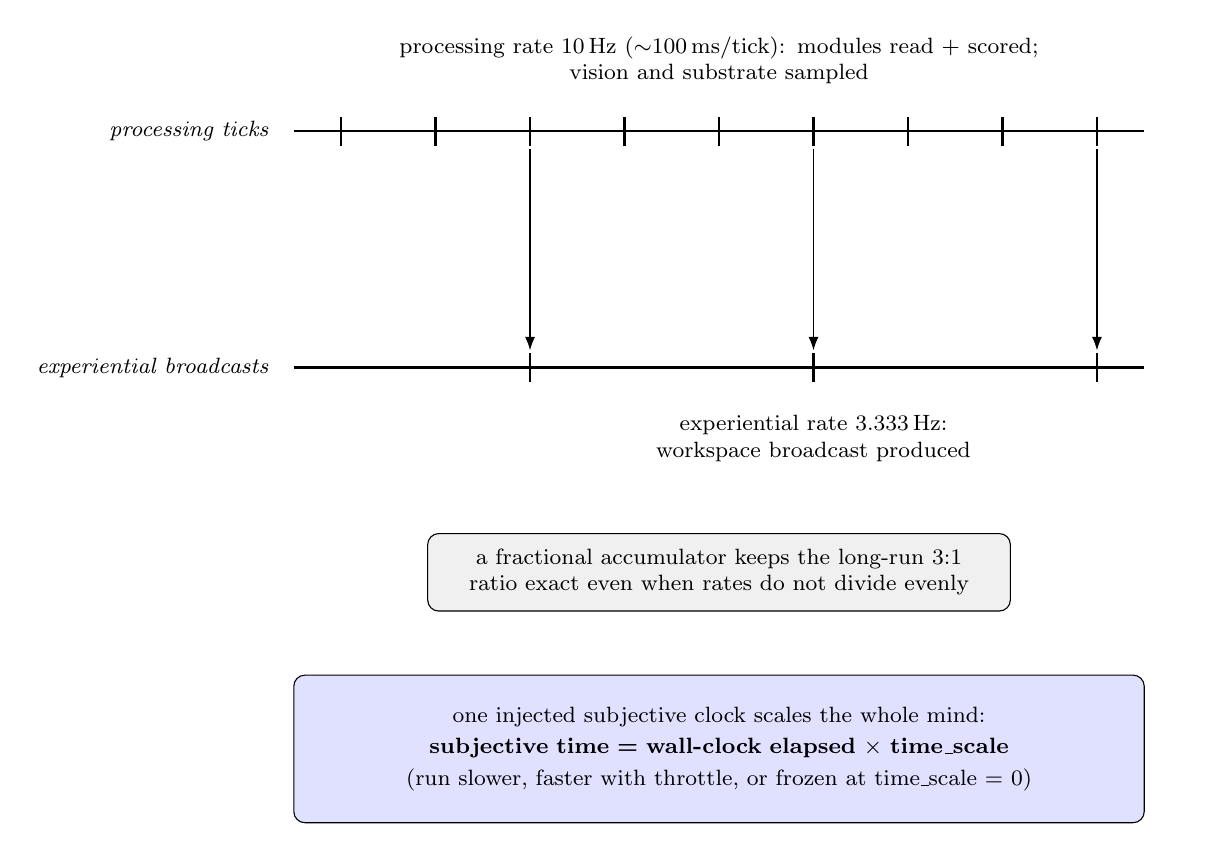
\begin{tikzpicture}[
  font=\small,>=Latex,
  tickmark/.style={draw, thick},
  capstyle/.style={draw, rounded corners, fill=blue!12, align=center, font=\footnotesize, text width=100mm, inner sep=4mm},
  notestyle/.style={draw, rounded corners, fill=gray!12, align=center, font=\footnotesize, text width=70mm, inner sep=2mm},
]

% --- upper track: processing ticks ---
\def\upy{3.0}
\def\loy{0.0}
\draw[thick] (-0.6,\upy) -- (10.2,\upy);
\foreach \i in {0,...,8} {
  \pgfmathsetmacro{\x}{\i*1.2}
  \draw[tickmark] (\x,\upy-0.18) -- (\x,\upy+0.18);
}
\node[align=center, font=\footnotesize, text width=115mm] at (4.8,\upy+0.9)
  {processing rate 10\,Hz ($\sim$100\,ms/tick): modules read $+$ scored;\\ vision and substrate sampled};

% --- lower track: experiential broadcasts ---
\draw[thick] (-0.6,\loy) -- (10.2,\loy);
\foreach \x in {2.4,6.0,9.6} {
  \draw[tickmark] (\x,\loy-0.18) -- (\x,\loy+0.18);
}
\node[align=center, font=\footnotesize, text width=70mm] at (6.0,\loy-0.9)
  {experiential rate 3.333\,Hz: workspace broadcast produced};

% --- arrows: every third processing tick feeds a broadcast tick ---
\foreach \x in {2.4,6.0,9.6} {
  \draw[->, thin] (\x,\upy-0.22) -- (\x,\loy+0.22);
}

% track labels
\node[font=\footnotesize\itshape, anchor=east] at (-0.8,\upy) {processing ticks};
\node[font=\footnotesize\itshape, anchor=east] at (-0.8,\loy) {experiential broadcasts};

% --- accumulator note, tucked below the lower-track label ---
\node[notestyle] at (4.8,-2.6) (acc)
  {a fractional accumulator keeps the long-run 3:1 ratio exact even when rates do not divide evenly};

% --- bottom caption spanning the width ---
\node[capstyle, below=8mm of acc] (capbox)
  {one injected subjective clock scales the whole mind:\\[2pt]
   \textbf{subjective time = wall-clock elapsed $\times$ time\_scale}\\[2pt]
   (run slower, faster with throttle, or frozen at time\_scale~$=$~0)};

\end{tikzpicture}
\end{document}
